\chapter{REVIEW}\label{ch:Review}

\section{SENSORS FOR OBSTACLE DETECTION}\label{sec:sensor}

\subsection{Overview}\label{sec:SensorOverview}

Many sensors can be used for obstacle detection such as ultrasonic
sensor, laser range finder, sonar, or image sensor, 3D flash LIDAR
\cite{de_angelis_low-cost_2007} \cite{alonge_novel_2009}
\cite{harb_neural_2008} \cite{saad_robust_2011}
\cite{williams_efficient_2001} \cite{chong_feature-based_1999}
\cite{hanna_obstacle_2008} \cite{lu_distance_2010}
\cite{civera_inverse_2008} \cite{jirawimut_visual_2003}
\cite{amzajerdian_lidar_2011}. Ultrasonic sensors such as radar and
sonar, and laser range finder are capable of providing high accuracy
range measurement up to centimeter level, but only provides point
measurement at a given position and orientation. To acquire a full 3D
range map of a scene, mechanical scanning mechanisms are required,
which limits the data acquisition rate of these device. LIDAR operate
in the same manner as laser range finder, except with the scanning
mechanism built in. Although LIDAR is becoming more and more popular
on land robot platform, it is usually expensive
\cite{subharsanan_low_2013} or have high power requirement and mass
when long range is required \cite{lemmens_airborne_2007}. Sonar is
usually used in indoor or under water applications, and have wide beam
profile which make it difficult to identify the origin of return
signal, and results in low resolution range map. 3D flash LIDAR is
capable of acquire 3D range measurement simultaneously by illuminating
the entire field of view of the camera with a single laser, and
capturing the reflected laser with a 2D imaging sensor
\cite{amzajerdian_lidar_2011}. However, its high cost has limited its
use in commercial application. In recent years, many researches use
optical sensor as a passive range sensor for its low weight, low cost.
With the help of computer vision technology, optical sensors have been
successfully used for range mapping and obstacle detection in a number
of platforms \cite{einhorn_cant_2010} \cite{hashimoto_detection_1996}
\cite{yamaguchi_moving_2006} \cite{zhang_obstacle_2012}
\cite{maier_self-supervised_2011} \cite{kubota_global_2007}
\cite{xu_method_2009} \cite{hanna_obstacle_2008}
\cite{zhang_real-time_2012} \cite{van_der_mark_stereo_2007}
\cite{broggi_stereo_2011}.

\subsection{Monocular Vision and Binocular Vision}
Image sensors are bearing-only sensors, which provide the measurement
on the direction of the features, and not the range. Other sensor
mentioned above, such as radar, LIDAR, are range and bearing sensor.
the principle of range measurement is through triangulating a common
scene point in two or more images captured. There are two types of
configuration in using optical sensor for range mapping through
triangulation: monocular, binocular. 

For binocular camera setups, two cameras are placed
apart from each other with their relative geometry (baseline
separation) known and captures images simultaneously. If the position
of a scene point can be accurately found in the images by both
cameras, its distance can be calculated by using the difference in
position of the projected point in images, and the separation of the
cameras. Because binocular setup acquires two images simultaneously,
the feature distance can be obtained at time 0. The challenge in
binocular range sensing is feature correspondence between the two
images. In addition, because of the limited distance in separation
between the camera, and the vibration noise caused by vehicle motion,
binocular range sensing are usually applied in short to medium range
measurement. 

For monocular camera setup, only one camera is used with an odometry
sensors providing camera displacement measurement between frames. Then
similar principle applies to triangulate the common scene point in two
frames to measurement the distance of the point. If camera is facing
the direction of travel, data association is less difficult as image
difference from frame to frame is usually small. Secondly, the
baseline separation can be selected according to the targeted object
distance by processing every frame, every other frames, or every n
frames captured which enable monocular camera being used for longer
range measurement. On the other hand, since monocular camera
configuration capture 1 frames at a time, the earliest range
measurement is available until two frames of images has been captured.

\subsection{Camera Calibration}

Camera model is what relating measurement on image plane to
measurement of the real world. Without it, measurement of the 3D world
through camera will be incorrect by a scale factor. Camera calibration
gives a model of the camera's geometry and a distortion model of the
lens. These models define the \textit{intrinsic parameters} of a
camera. 

\subsubsection{Basic Projection Geometry}

For a 3D scene point $Q=(X, Y, Z)$ and the correspondent point $q=(x_{screen},
y_{screen})$ on the image plane, they are related by equation \cite{learning_opencv}

\begin{equation}
\begin{matrix}
x_{screen} = f_x\left(\frac{X}{Z}\right)+c_x, &
y_{screen}=f_y\left(\frac{Y}{Z}\right)+c_y
\end{matrix}
\end{equation}

\noindent where $(c_x, c_y)$ is the image plane coordinate at which optical axis
intersects the image plane, $f_x$ and $f_y$ is the product of focal
length $f$ (unit millimeter) with the scaling factor $s_x$ and $s_y$
(unit pixel/millimeter) for X and Y. Therefore $f_x$ and $f_y$ is in
unit pixel. The parameter $c_x$, $c_y$, $f_x$, $f_y$ define the camera
intrinsics matrix \cite{learning_opencv} \cite{Heikkila_four_1997}.

\begin{equation}
M = \begin{bmatrix}
f_x & 0 & c_x \\
0& f_y & c_y \\
0 & 0 & 1 \end{bmatrix}
\end{equation}

\subsubsection{Lens Distortion}
There are two main contributor to lens distortion. Radial distortion
and tangential distortion. Radial distortion arise as a result of the
shape of lens. It cause noticeable distortion to the pixels close to
the edge of the imager, resulting in ``fish-eye'' effect. The radial
distortion is zero at the center of the imager, and increases with the
distance to the optical center. It is characterized by the first few
terms of a Taylor series expansion

$$ x_{corrected} = x(1+k_1r^2+k_2r^4+k_3r^6)$$
$$ y_{corrected} = y(1+k_1r^2+k_2r^4+k_3r^6)$$

\noindent Tangential distortion arise from the misalignment
between the image sensor and the lens. It is minimally characterized
by two additional parameters $p_1$ and $p_2$

$$x_{corrected} = x+[2p_1y+p_2(r^2+2x^2)]$$
$$y_{corrected} = y+[p_1(r^2+2y^2)+2p_2x]$$

\subsubsection{Camera Calibration Algorithm}

\subsection{Limitation of Optical Sensor in Recursive Algorithm}
\label{sec:OpticalSensorLimitation}

\begin{itemize}
  \item Error Accumulation over Iterations
  \begin{itemize}
    \item Feature quality Decreases over Iterations
  \end{itemize}
\end{itemize}

\subsection{GPS and IMU}\label{sec:gps_and_imu}
GPS and IMU are generally available on UAVs. These sensors provide a 
measurement on the robot motion. Odometry can provide the scale 
information which is missing in the bearing only measurement. 
Furthermore, odometry provides some prior information on the robot 
motion which can help to disambiguate the solution.

\section{SLAM as A Sensor Fusion Framework}
\label{sec:SLAM}
An essential aspect of autonomy for a mobile robot is the capability to 
determine its location. This capability is known as localization. 
Localization is typically a prerequisite for accomplishing real tasks, 
whether it is exploration, navigation toward a known goal, 
transportation of material, construction or site preparation. In many 
applications, the mobile robot has an a priori map. Given a map, the 
robot may localize by matching current sensor observations to features 
in the map. Given enough features and an unambiguous geometry, the pose 
of the robot can be determined or at least narrowed down to a set of 
possible locations.

Usable maps do not always exist, and it is not always possible to have 
accurate externally referenced pose estimates. If an a priori map is not 
available, the robot may need to construct one. With a precise, 
externally referenced position estimate from GPS or similar means, the 
robot can take its sensor observations, reference the observations to 
its current pose, and insert features in the map in the appropriate 
places. Without maps or externally referenced pose information, the 
robot must produce its own map and concurrently localize within that 
map. This problem has been referred to as concurrent localization and 
mapping (CLM) and simultaneous localization and mapping (SLAM).

\subsection{Recursive Probabilistic Estimation using Extended Kalman Filter}
\label{sec:SLAM_using_EKF}

The Kalman filter \cite{kalman_new_1960}published by R. E. Kalman in
1960 is a very powerful recursive data processing algorithm for
dynamic stochastic processes. The filter find extensive use in control
and navigation application for its ability of estimating past, present
and even future state. It is an attractive candidate for data fusion
framework as it can process all available measurements including
previous knowledge of the process, regardless of their precision, to
estimate the current value of the variable of interest. Given a
dynamic process that satisfy the assumptions that Kalman filter is
based on, the filter is the optimal algorithm in minimzing the mean of
squared error of the state variable. This section briefly summerized
assumption and formation of Kalman filter that's described in detail
in \cite{sorenson_least-squares_1970}
\cite{analytic_sciences_corporation_applied_1974}
\cite{grewal_kalman_1993} \cite{lewis_optimal_1986}
\cite{brown_introduction_1993}. A more intuitive introduction can be
found in chapter 1 of \cite{maybeck_stochastic_1979}.
%reference in Welch and bishop
% intro to Kalman filter.

The Kalman filter has three assumptions. 1) The system model is
linear. The linearity is deisred in that the system model is more
esily manipulated with engineering tool. When nonlinearities do exist,
the typical approach is to linearize system model at some nominal
points. 2)The noise embedded in system control and measurement is
white. This assumption implies that the noise value is not correlated
in time, and has equal power in all frequency. 3)The probability
density function (PDF) of system and measurement noise is Gaussian. A
Gaussian distribution is fully represented by the first and second
order statistic (mean and variance) of a process. Most other densities
require endless number of orders of statistic to describe the shape
fully. Hence, when the probability density function of a noise process
is non-Gaussian, the Kalman filter that propagates the first and
second order statistic only include some of the information of the
PDF, instead of all, as would be the case with Gaussian noise.

\subsubsection{Kalman Filter Models}
The Kalman filter requires two models. The process model define a
discrete-time controlled process by a linear stochastic difference
equation. The $n\times n$ matrix $A$ relates the state variables
$x_{k-1}$ in previous time step $k-1$ to the state variabl $x_{k}$ in
the current time step $k$. The matrix $B$ relates the optional control
input $\mu$ to the state variables $x$. Given measurement vecor $z_k$
of size $1 \times m$, the measurement model relates the state
variables to the measurements by matrix H of size $n \times m$. The
random variable $w$ and $v$ represent the uncertainty or noise of the
process model, and measurement. $w$ and $v$ are assumed to be
unrelated to each other, and has Gaussian distribution with covariance
$Q$ and $R$. 

\begin{align}
&\text{Process Model: }x_k = Ax_{k-1}+B\mu_{k-1}+w_{k-1}\\
&\text{Measurement Model: }z_k = Hx_k+v_k
\end{align}

\subsubsection{The Algorithm}
The Kalman filter operates in prediction and correction cycle after
being initialized \ref{figch2:1}, with the state vector estimate
$\hat{x}^-_k, \hat{x}^+_k$ contains the variable of interest at time
step k, and state covariance matrix $P^-_k, P^+_k$ representing the
error covariance of the estimate. The superscript - indicate the
estimate is a priori (or predicted) estimate, and + indicate the
estimate is a posteriori (or corrected) estimate. The equations used
for prediction and correction are listed in \ref{tab:KF}. In
prediction, an estimate of the state variables are made based on the
known knowledge of the process (the process model). Since there are
always unknown factor not fully described by the process model, the
error of the estimate almost always increase in the prediction. During
correction, a series of calculation were carried out to correct the a
priori estimate. First, the predicted measurement $H\hat{x}^-_k$ are
compared to the new measurement $z_k$. Their difference $z_k -
H\hat{x}^-_k$ is called the measurement innovation, or residual. Next,
the amount of residual is weighted by the Kalman gain $K$, and added
to $\hat{x}^-_k$ as correction. The Kalman gain is fomulated so that
it minimize the a posteriori error covariance matrix $P^+_k$. 

\begin{figure}[h]
\centering
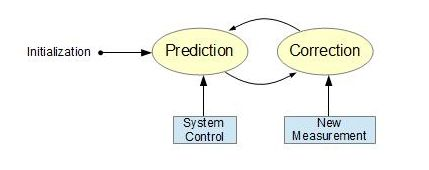
\includegraphics[width=10cm, keepaspectratio=true]{./Figures/KalmanOperation.jpg}
\caption{Kalman Operation Flow Diagram}
\label{figch2:1}
\end{figure}

\begin{table}
\caption{Kalman Filter Operation Equations}
\label{tab:KF}
\centering
\begin{tabular}{|l|c r|}
\hline
\multirow{2}{*}{Prediction} 
& $\hat{x}^-_k=A\hat{x}^+_{k-1}+B\mu_{k-1}$ & \stepcounter{equation}\thetag{\theequation}\\
& $P^-_k = AP^+_{k-1}A^T+Q$ & \stepcounter{equation}\thetag{\theequation}\\
\hline
\multirow{3}{*}{Correction}
& $K_k=P^-_kH^T(HP^-_kH^T+R)^{-1}$  & \stepcounter{equation}\thetag{\theequation}\\
& $\hat{x}^+_k = \hat{x}^-_k+K_k(z_k-H\hat{x}^-_k)$ & \stepcounter{equation}\thetag{\theequation}\\
& $P^+_k = (I-K_kH)P^-_k$ & \stepcounter{equation}\thetag{\theequation}\\
\hline
\end{tabular}
\end{table}
\FloatBarrier

\subsubsection{Extended Kalman Filter}
For a discrete-time controlled process, or its relationship with the
measurements are non-linear, a Kalman filter must be linearized about
the estimated trajectory, and is referred to as an extended Kalman
filter or EKF. A process with state vector $x$ and measurement $z$
that is governed by non-linear stochastic difference equation has
process and measurement model 
\begin{equation}
x_k=f(x_{k-1}, u_{k-1}+w_{k-1}),
\end{equation}
\begin{equation}
z_k=h(x_k+v_k),
\end{equation}
\noindent where the random varialbe $w_k$ and $v_k$ represent the
process and measurement noise with variance $Q$ and $R$. The the
Kalman filter operation equations are given in table
\ref{tab:EKF},

\begin{table}[H]
\caption{Extended Kalman Filter Operation Equations}
\label{tab:EKF}
\centering
\begin{tabular}{|l|c r|}
\hline
\multirow{2}{*}{Prediction} 
& $\hat{x}^-_k=f(\hat{x}^+_{k-1},\mu_{k-1},0)$ & \stepcounter{equation}\thetag{\theequation}\\
& $P^-_k = A_kP^+_{k-1}A_k^T+W_kQ_{k-1}W_k^T$ & \stepcounter{equation}\thetag{\theequation}\\
\hline
\multirow{3}{*}{Correction}
& $K_k=P^-_kH_k^T(H_kP^-_kH_k^T+V_kR_kV_k^T)^{-1}$  & \stepcounter{equation}\thetag{\theequation}\\
& $\hat{x}^+_k = \hat{x}^-_k+K_k(z_k-h(\hat{x}^-_k,0))$ & \stepcounter{equation}\thetag{\theequation}\\
& $P^+_k = (I-K_kH)P^-_k$ & \stepcounter{equation}\thetag{\theequation}\\
\hline
\end{tabular}
\end{table}
\FloatBarrier

\noindent where (subscript $k$ omitted)
\begin{itemize}
  \item $A$ is the Jacobian matrix of partial derivatives of $f$ with
  respect to $x$, $$A_{[i,j]}= \frac{\partial f_i(\hat{x}_{k-1}^+, \mu_{k-1},
    0)}{\partial x_j}$$
  \item $W$ is the Jacobian matrix of partial derivatives of $f$ with
  respect to $w$, $$W_{[i,j]}= \frac{\partial f_i(\hat{x}_{k-1}^+, \mu_{k-1},
    0)}{\partial w_j}$$
  \item $H$ is the Jacobian matrix of partial derivatives of $h$ with
  respect to $x$, $$H_{[i,j]}= \frac{\partial h_i(\hat{x}_k^-, 0)}{\partial x_j}$$
  \item $V$ is the Jacobian matrix of partial derivatives of $h$ with
  respect to $v$, $$V_{[i,j]}= \frac{\partial h_i(\hat{x}_k^-,0)}{\partial v_j}$$
\end{itemize}

\noindent Note that when $w$ and $v$ directly describe the noise of
state vector and measurement, the table \ref{tab:EKF} is the same as
table \ref{tab:KF}. 

\subsubsection{Tuning}

The tuning of the filter can be achieved by adjusting noise covariance
matrix $Q$ and $R$. The measurement noise covariance $R$ is usually
easy to estimate, ie., by taking some offline measurements to compute
the variance. On the other hand, process noise covariance $Q$ is more
difficult. One common way is to inject enough uncertainty into the
process noise, and only rely on reliable measurements. 
 
\subsection{SLAM with Extended Kalman Filter}

The simultaneous localization and mapping(SLAM) problem answers to
whether a robot can be make truly autonomous if it is plaed at an
unknown location in an unknown environment. AFter many decades of
research, the stucture of SLAM problem now has evolved to a standard
Bayesian form. Two key approaches to solving a SLAM problem is to use
the extended Kalman filter (EKF-SLAM) and through the use of
Rao-Blackwellized particle filter (FastSLAM). A thourough tutorial to
the SLAM problem is given in \cite{durrant-whyte_simultaneous_2006}
\cite{bailey_simultaneous_2006}.

\subsubsection{General EKF Model for SLAM}
There is a high degree of correlation betwee the estimates of the
location of the landmarks in map \cite{smith_representation_1986}
\cite{durrant-whyte_uncertain_1988}. This correlation exists because
of the common error in the estimated vehicle location
\cite{leonard_simultaneous_1991}. The implication of these works is
that a consistent full solution to the SLAM problem require a joint
state composed of the vehicle pose and every landmark position
\cite{durrant-whyte_simultaneous_2006}. When the vehicle pose and
landmarks position are fomulated as one single estimation problem, the
result was convergent. The correlation between landmark play an
important role in the quality of the solution. The more these
correlation grew, the better the solution.
\cite{durrant-whyte_localization_1996} \cite{csorba_new_1996}
\cite{csorba_simultaneous_1997} \cite{dissanayake_solution_2001}

At a given time step $k$, the following variables are defined
\begin{itemize}
  \item $x_k$ describe the vehicle position and orientation.
  \item $u_k$ the control vector applied at time $k-1$ to drive the
  vehicle to $x_k$ at time k
  \item $p_i$ a vector desecribe the location of the ith landmark. All
  landmarks locations are assumed to be time invariant.  
  \item $z_{ik}$ observation of the location of the ith landmark taken
  from the vehicle's location at time $k$
\end{itemize}

Then a complete state vector contains
$$\begin{bmatrix}\hat{x}_k \\ \hat{p}_k \end{bmatrix}$$
\noindent and the state covariance matrix contains
$$\begin{bmatrix}
P_{xx} & P_{xp} \\
P_{px} & P_{pp} 
\end{bmatrix} $$

The prediction and correction procedure can then be carried out
following the standard EKF formulation. The lamdmarks are generally
not updated at the prediction (ie. only $x_k$ and $P_{xx}$ are
updated) unless they are moving.

\subsubsection{Properties of SLAM}
\label{sec:SLAM_properties}

Dissanayake \cite{dissanayake_solution_2001} reached three important
convergency properties of Kalman filter based SLAM, namely that: 
\textit{
\begin{enumerate}
  \item the determinant of any submatrix of the map covariance matrix
  decreases monotonically as observations are successively made;
  \item in the limit as the number of observations increases, the
  landmark estimates become fully correlated;
  \item in the limit the covariance associated with any single
  landmark location estimate reaches a lower bound determined only by
  the initial covariance in the vehicle location estimate at the time
  of the first sighting of the first landmark.
\end{enumerate}}

These result shows that the complete knowledge of cross correlation
between landmark estimates is critical in maintaining the structure of
a SLAM problem. The error in estimates of landmarks becomes more and
more correlated as the vehicle venture throuth the unknown
environment. The error eventually becomes fully correlated which means
given the location of one landmark, the location of any other landmark
can be determined with absolute certainty. As the map converges, the
error in the estimates of landmarks reduce to a lower bound determined
by the error when the first observation was made. 

The results above only refer to the evolution of covariance matrices
computed by linear model. In reality, SLAM problem is nonlinear, and
the computed covariance does not match the true estimation error. This
leads SLAM consistency issue.

\subsubsection{Linearization Error and Consistency}

Many researches reported and analyzed filter divergence due to
linearization error \cite{martinelli_results_2005},
\cite{julier_counter_2001}, \cite{bailey_consistency_2006},
\cite{frese_discussion_2006}, \cite{castellanos_limits_2004}. As
defined in \cite{huang_analysis_2008}, a state estimator is consistent
if the estimation errors (i) are zero-mean, and (ii) have covariance
matrix smaller or equal to the one calculated by the filter.

Huang investigated \cite{huang_convergence_2007} on properties and
consistency of nonlinear two-dimensional EKF based SLAM problem,
derived and proved a number of theorem applied to EKF SLAM convergence
and consistency issue, and concluded:

\begin{itemize}
  \item Most of the convergence properties in
  \cite{dissanayake_solution_2001} are still true for the nonlinear
  case provided that the Jacobians used in the EKF equations are
  evaluated at the true states.
  \item The main reasons for inconsistency in EKF SLAM (over
  optimistic estimation) are due to 
  \begin{enumerate}
    \item the violation of some fundamental constraints governing the
    relationship between various Jacobians when they are evaluated at
    the estimated location, instead of the true location
    \item the use of relative location measurements from robot to
    landmarks to update the absolute robot and landmark location
    estimates in world coordinate.
  \end{enumerate}
  \item The robot orientation uncertainty plays an important role in
  both the EKF SLAM convergence and the possible inconsistency. 
\end{itemize}

\subsubsection{SLAM for Building Large Scale Maps}

\paragraph{Robot Centric Coordinate System}In response to the
consistency problem of classic EKF SLAM solution, some research
adopted the \emph{robotcentric mapping} \cite{castellanos_limits_2004}
\cite{civera_1-point_2009}. This approach uses a reference frame
attached to the robot as the base frame. All geometric measurements
and estimations are referred to the robot frame. This method was shown
to improve the consistency of EKF based solution to SLAM, but using
local map joining to produce a large map gives better result. 

\paragraph{Submap Methods}The submap methods are another mean to
tackle large scale map problem. The submaps can be either globally
referenced or relatively referenced. Global submaps estimate the
location of the submap referenced to a common base frame
\cite{estrada_hierarchical_2005} \cite{leonard_consistent_2003}.
However, as the submap frames are referred to a common base frame,
global submap does not improve the consistency issue caused by the
robot pose uncertainty.\cite{bailey_simultaneous_2006}. Relatively
referenced submap record its location referenced to the neighboring
submaps \cite{chong_feature-based_1999}
\cite{williams_efficient_2001}. Global map is then obtained through
vector summation. The relative submap is able to alleviate
linearization problem in large scale map, but does
not converge on global level without an independent submap structure.
This problem can be solved by using Atlas framework and network
coupled feature maps \cite{bosse_slam_2004} \cite{bailey_mobile_2002}
%%% Local Variables:
%%% mode: latex
%%% TeX-master: "thesis"
%%% End:





